\documentclass{article}
\usepackage{tpack}
\pgfplotsset{compat=newest}
\usetikzlibrary{patterns}
\begin{document}
    \begin{figure}[H]
        \centering
        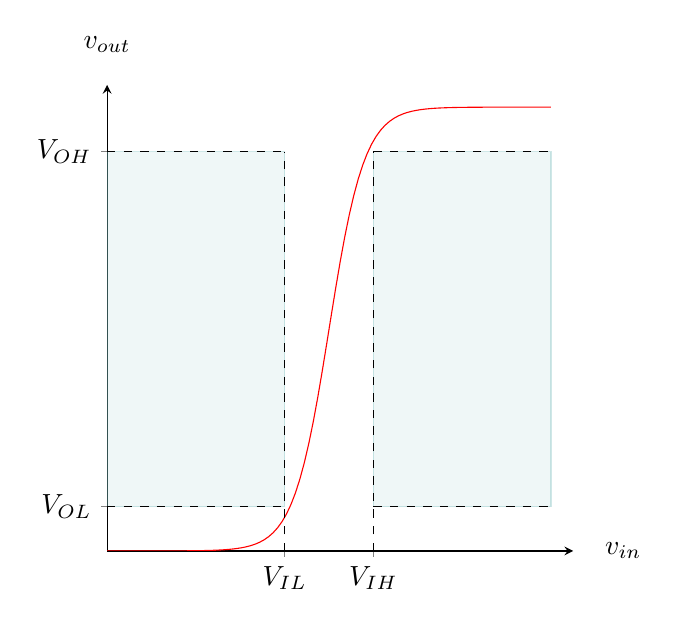
\begin{tikzpicture}
            \begin{axis}[
                xmin = 0, xmax = 5.25, % Axis Coordenates
                ymin = 0, ymax = 5.25, % Axis Coordenates
                xlabel = {$v_{\text{in}}$},  % Axis Labels
                ylabel = {$v_{\text{out}}$}, % Axis Labels
                xtick = {2,3},      % Axis Ticks Potions
                ytick = {0.5,4.5},  % Axis Ticks Potions
                xticklabels = {$V_{IL}$, $V_{IH}$}, % Axis Ticks Labels
                yticklabels = {$V_{OL}$, $V_{OH}$}, % Axis Ticks Labels
                x label style = {at={(axis cs:{5.5,0})}, anchor=west},
                y label style = {at={(axis cs:{0,5.5})}, anchor=south, rotate=-90},
                width  = 7.5cm,
                height = 7.5cm,
                % grid = both,
                % grid style       = {line width=.1pt, draw=gray!10},
                % major grid style = {line width=.2pt, draw=gray!50},
                % minor tick num=1,
                axis lines = left,
            ]
            \addplot [
                    domain=0:5, 
                    samples=100, 
                    color=red,
            ] {5/(1+exp(-5*x+12.5))};
            \draw[
                color   =teal!75,
                fill    =teal!25,
                opacity =0.25
            ] (3,0.5) rectangle (5, 4.5);
            \draw[
                color   =teal!75,
                fill    =teal!25,
                opacity =0.25
            ] (0,0.5) rectangle (2, 4.5);
            \draw[dashed] (axis cs:{2,0}) -- (axis cs:{2,4.5});
            \draw[dashed] (axis cs:{3,0}) -- (axis cs:{3,4.5});
            \draw[dashed] (axis cs:{0,0.5}) -- (axis cs:{2,0.5});
            \draw[dashed] (axis cs:{3,0.5}) -- (axis cs:{5,0.5});
            \draw[dashed] (axis cs:{0,4.5}) -- (axis cs:{2,4.5});
            \draw[dashed] (axis cs:{3,4.5}) -- (axis cs:{5,4.5});
            \end{axis}
        \end{tikzpicture}
    \end{figure}\noindent
\end{document}